% !TEX root = ../Thesis.tex

%requirements plusminus 2 pagina's
\section{Objectives (R-M)}
\label{sec:objectives}
In this section we give an overview of the most important objectives of this graduation project, along with an introduction to the project and its context.
The complete list of objectives as given in the beginning of the project is given in the project planning \citepr{plan}.
% !TEX root = ../Thesis.tex

\subsection{Ampersand project}
In November 2003, the Business Rules Manifesto \citenac{business-rules} was published by the Business Rules Group, with the main purpose of declaring independence for business rules in the world of requirements.
The manifesto supports the vision of business rules as equivalent to requirements.
This is considered a radical change on how people see the world of business architecture \citeac{ross_bra}. 

In December 2010, Stef Joosten, Lex Wedemeijer and Gerard Michels published the paper `Rule Based Design', presenting the Ampersand approach.
The approach puts the rules in the center, using these rules to define the business processes.
Ampersand is named after the \& symbol with the desire of realizing results for both business and IT, in an efficient and effective way.

In 2011, the Ampersand compiler was created as an open source project.
Since then, the compiler has been improved and applied in both business and academic contexts.
The Ampersand end-users write business rules in a domain specific language (ADL), and compile that specification into functional specification, documentation and working software prototypes.
\dict{ADL}{Ampersand Definition Language}%
These rules are based on agreements between the different stakeholders.

The theory behind Ampersand has been thoroughly studied, and is based on mathe\-matical concepts, e.g. relational algebra and Tarski's axioms.
Using the Ampersand compiler, users write the requirements in ADL and generate all the system specification independent of the platform.
The main advantage is that the requirements' consistency and traceability are always correct (and even provable), from the lowest level up to the front-end.
The requirements are presented to stakeholders in natural language, guaranteeing that any business expert who knows the context can validate the requirements.
\autoref{fig:generation} depicts the artifacts generated by the Ampersand compiler.
%
\begin{figure}[htb]
	\centering
	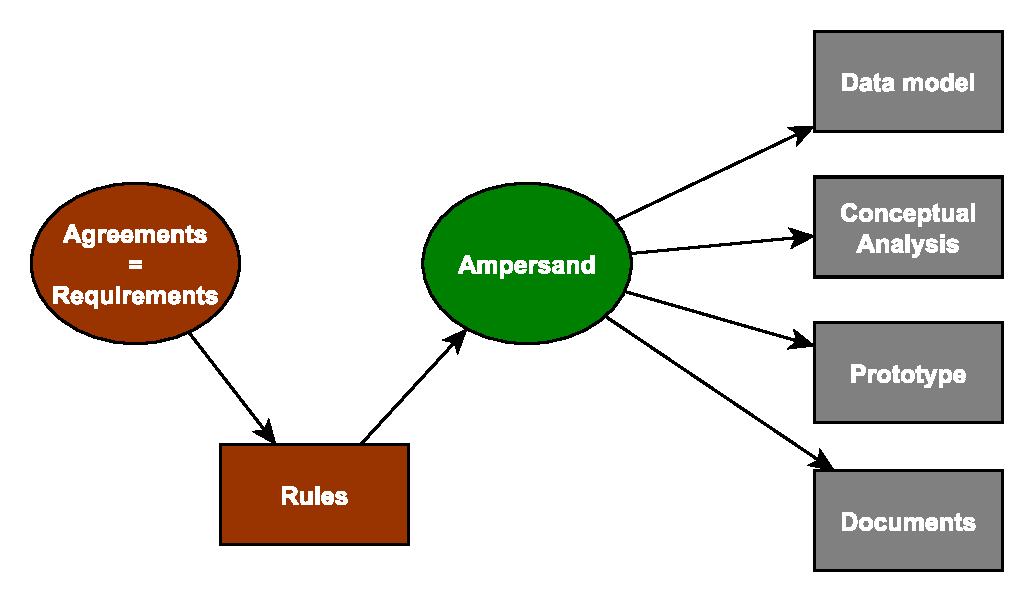
\includegraphics[width=0.7\textwidth]{Figures/Generation}
	\caption[Generated artifacts]{Ampersand generates several artifacts based on the business rules (source: \cite{ampersand-approach})}
	\label{fig:generation}
\end{figure}
%

The Ampersand project is used in several environments, by different user groups.
In a research context, the Ampersand project is part of the research on the use of business rules for software design.
In an educational context, it is also used as the main tool in the course `Rule Based Design' from the Open University of the Netherlands.
Finally, the compiler is used in business environments to design and develop real world business software.

% !TEX root = ../Thesis.tex

\subsection{High-level architecture}
\label{subsec:architecture}
The compiler developed for the Ampersand research project runs in several steps, hence the Ampersand compiler is also divided in several subcomponents:
\dict{P-structure}{The parse-tree generated by the Ampersand parser, used as input for the type checker}%
\dict{A-structure}{The ADL code generated by the Ampersand type checker, used as input for the calculator component}%
\dict{ADL-structure}{See A-structure}%
\dict{F-structure}{The functional structure generated by the Ampersand calculator, used as input for the different output modules}%
\begin{itemize}
	\item \textbf{Parser}: This component receives the ADL code as input, and parses that code into a parse-tree (also known as P-structure).
	\item \textbf{Type checker}: The Ampersand type checker receives a P-structure as input and converts it into a relational algebra format, suitable for manipulation (also known as A-structure or ADL-structure).
		 The semantics of ampersand are expressed in terms of the A-structure.
	\item \textbf{Calc}: The Calc component receives an A-structure as input, and manipulates it according to the research rules, generating the functional structure (also known as F-structure).
		The F-structure contains all design artifacts needed to write a specification and generate the output.
	\item \textbf{Output components}: All design artifacts present in the F-structure are ready to be rendered.
		Several components use this data structure to generate the wished output.
		The output components currently implemented (and their output formats) are the following: 
		\begin{itemize}
			\item Atlas (HTML interface);
			\item Revert (Haskell source);
			\item Query (prototype generation);
			\item Documentation Generator (Pandoc structure).
		\end{itemize}
\end{itemize}

% !TEX root = ../Documentation.tex

\subsection{Parser (R-M)}
\label{subsec:design-parser}
The mainstream design of the new parser has not changed much.
Basically, each EBNF rule receives its own parser function.
Thanks to the combinator operators, each parsing function also looks very similar to its corresponding EBNF.

The applicative interface is consistently used.
By changing details of the implementation, e.g. the order of the fields in the parse tree, we have made many of the `rebuild' functions unnecessary.
For some parsers the amount of changes necessary in order to remove supporting functions was too large or even impossible with the current parse tree.

Note that in parts of the parser, the function syntax has substituted the record syntax for creating data objects.
This was done only when the code readability could be improved by doing so.

\subsubsection{Parsec}
\label{subsec:design-parsing-lib}
As mentioned earlier, and described in research context document \citenac{parsing}, the new Ampersand parser has been rebuilt with another parsing library, namely Parsec.
However, for the Ampersand developers, the source code of the parser will still look very familiar, thanks to the applicative interface.
For developers, the main differences between Parsec and the uulib are:
\begin{itemize}
  \item Parsec does not backtrack by default.
    In order to enable backtracking, the \texttt{try} function must be used.
    This is described in \autoref{subsec:backtracking}.
  \item Parsec does not try to solve parsing errors.
    The parser stops immediately after the first issue.
    See also the error analysis in \autoref{subsec:design-errors}.
  \item Error messages are customizable by using the \texttt{<?>} operator.
    This is also suggested in \autoref{subsec:design-next-steps}.
  \item Some combinators have a different name, e.g. one must use \texttt{option} instead of \texttt{opt}.
    Assuming the documentation found on Hackage is clear and sufficient, interface differences are not documented here.
\end{itemize}

\subsubsection{Backtracking}
\label{subsec:backtracking}
In order to explain the differences on backtracking behavior between the uulib and Parsec, we quote here Doaitse Swierstra, the author of the uulib \citenac{swierstra-parsec}:
\begin{quote}
\textsl{To understand the subtleties it is important to understand the differences between the try construct in Haskell and the non-greedy parsing strategy used in uu-parsinglib. Effectively the latter is a try which just looks ahead one symbol. In that respect it is less powerful than the try construct from Parsec, in which you specify that a specific construct has to be present completely. And then there is the underlying different overall strategy. Parsec uses a back-tracking strategy with explicit tries to commit, whereas uu-parsinglib uses a breadth-first strategy with an occasional single symbol look-ahead.}
\end{quote}
%
We can therefore conclude that the try-statements in Parsec are undesirable.
However, they are necessary when the grammar is ambiguous.
In this section we explain why each of the remaining try statements are necessary, and how these issues can be resolved:
\begin{description}
  \item[Classify]
    This ambiguity in the grammar arises from the \texttt{Classify} and \texttt{GenDef} productions:
    \begin{quote}
        \texttt{Classify ::= `CLASSIFY' ConceptRef `IS' Cterm}\\
        \texttt{GenDef ::= (`CLASSIFY' | `SPEC') ConceptRef `ISA' ConceptRef}
    \end{quote}
    When the parser encounters \texttt{`CLASSIFY'}, it cannot define whether it found a \texttt{Classify} or a \texttt{GenDef} production.
    Therefore, the parser must consume the keyword and a \texttt{ConceptRef} before consuming either \texttt{`IS'} or \texttt{`ISA'} and determining which production is applicable.
    
    In order to solve this issue, one must choose a different keyword or symbol for each of the productions.
    Another option would be to merge the two statements in the same parser.
    We did not merge the productions because that would make the parser less maintainable.
  
  \item[Role]
    This ambiguity in the grammar arises from the \texttt{RoleRelation} and \texttt{RoleRule} productions:
    \begin{quote}
        \texttt{RoleRelation ::= `ROLE' RoleList `EDITS' NamedRelList}\\
        \texttt{RoleRule ::= `ROLE' RoleList `MAINTAINS' ADLidList}
    \end{quote}
    When the parser encounters \texttt{`ROLE'}, it cannot define whether it is a \texttt{RoleRelation} or a \texttt{RoleRule} production.
    Therefore, the parser must consume the keyword and a \texttt{RoleList} (which may be long) before consuming either \texttt{`MAINTAINS'} or \texttt{`EDITS'} and determining which production is applicable.
    
    In order to solve this issue, one must choose a different keyword for each of the productions, merge the two options to have the same representation in the parse tree, or refactor the parser so that the two options are parsed together.
    We did not merge the productions because that would make the parser less maintainable.
  
  \item[View]
    This ambiguity in the grammar arises from the \texttt{FancyViewDef} and \texttt{ViewDefLegacy} productions:
    \begin{quote}
        \texttt{FancyViewDef ::= `VIEW' Label ConceptOneRefPos `DEFAULT'? `\{' ViewObjList `\}' HtmlView? `ENDVIEW'}\\
        \texttt{ViewDefLegacy ::= (`VIEW' | `KEY') LabelProps ConceptOneRefPos `(' ViewSegmentList `)' }
    \end{quote}
    When the parser encounters \texttt{`VIEW'}, it cannot define whether it found a \texttt{FancyViewDef} or a \texttt{ViewDefLegacy} production.
    In this case, defining which construction is applicable is even more complicated.
    This decision must, in the worst case, be delayed until the parser encounters a \texttt{`\{'} or \texttt{'('}.
    That's because the productions \texttt{Label} and \texttt{LabelProps} are not disjoint, and \texttt{`DEFAULT'} is optional.
    
    In order to solve this issue, we advise to merge or drop the legacy statement.
    
  \item[Multiplicity]
    This ambiguity in the grammar arises from the \texttt{Mult} production:
    \begin{quote}
        \texttt{Mult ::= (`0' | `1') `..' (`1' | `*') | `*' | `1'}
    \end{quote}
    When the parser encounters \texttt{`1'}, it cannot define whether it found the first or the last production.
    The parser must therefore read the next token before choosing the right option.
    
    In order to solve this issue, we advise to refactor the grammar (and the parser) to have the following production:
    \begin{quote}
        \texttt{Mult ::= `0' `..' (`1' | `*') | `1'(`..' (`1' | `*'))? | `*'}
    \end{quote}
    %
    We did not refactor the code in this manner because the \texttt{pMult} parser does more than only parsing: it also changes the representation of the found constructions before creating the parse tree.
  
  \item[Labels and Terms]
    In the productions \texttt{Att} and \texttt{RuleDef}, we see very similar ambiguities:
    \begin{quote}
        \texttt{Att ::= LabelProps? Term}\\
        \texttt{RuleDef ::= `RULE' Label? Rule Meaning* Message* Violation?}
    \end{quote}
    Wherein:
    \begin{quote}
        \texttt{Label ::= ADLid ':'}\\
        \texttt{LabelProps ::= ADLid (`{' ADLidListList `}')? `:'}\\
        \texttt{Rule ::= Term ('=' Term | '|-' Term)?}
    \end{quote}
    And one of the possible productions of \texttt{Term} is:
    \begin{quote}
        \texttt{Term ::= Trm2 ::= Trm3 ::= Trm4 ::= Trm5 ::= Trm6 ::= RelationRef ::= NamedRel ::= Varid Sign?}
    \end{quote}
    While:
    \begin{quote}
        \texttt{ADLid ::= Varid | Conid | String}
    \end{quote}
    
    What happens here is that when the parser encounters a \texttt{Varid}, it cannot define whether it is part of the (optional) \texttt{Label} production or if no \texttt{Label} was given and the \texttt{Varid} is part of a \texttt{Term}/\texttt{NamedRel} production.
    
    Due to the quite complex grammar for the \texttt{Term} production, this issue may severely impact the parser's performance.
    This is probably the most harmful of the ambiguities mentioned.
    However, it can only be solved by adding a symbol before the \texttt{Term} production (e.g. making the `:' non-optional).
\end{description}
%
Please note that in order to have proper backtracking with correct error messages, Parsec may require two try-statements \citenac{try-harmful}.

% !TEX root = ../Thesis.tex

\subsection{Other objectives}
While designing and implementing the new Ampersand parser, the following objectives were also important:
\begin{itemize}
  \item \textbf{Integration}: The new parser must interface with the remaining Ampersand modules.
    It must thus be implemented in Haskell.
  \item \textbf{Libraries}: Since different implementation options are available, it was important to choose the most suitable Haskell parsing framework.
  \item \textbf{Maintainability}: Well-written and maintainable code is a must for the Ampersand project, since it is an open-source project.
    The maintainability must be either maintained or improved; otherwise the parser is not to be taken into production.
  \item \textbf{Tests}: Testing the parser well was a task for this project.
    The suggestion is to use testing tools to improve the process, e.g. QuickCheck.
  \item \textbf{Pretty-printing}: This is important in order to test the parser.
\dict{HPC}{Haskell Program Coverage}%
\dict{Haddock}{Software documentation generator for the Haskell programming language}%
\dict{HLint}{Statical analysis software that suggests maintainability improvements}%
  \item \textbf{Tools}: Within the Haskell community, several tools are popular to verify code quality and generate documentation, e.g. HPC, Haddock and HLint.
  \item \textbf{Fixed syntax}: The new parser must process the same inputs as the previous parser.
  \item \textbf{Fixed parse tree}: The new parser must produce the same outputs as the previous parser.
    Any further changes must be applied to the rest of the Ampersand system.
\end{itemize}

During the project, some additional requirements have been identified:
\begin{itemize}
  \item \textbf{Git/GitHub}: The changed software had to be integrated into the GitHub Ampersand project.
    The development itself happened in a separate branch of a separate fork, so that deliveries could be merged in a smooth way.
    This was an especially hard requirement for us, since we had no experience with Git.
  \item \textbf{Cabal}: The building system for Haskell had to be maintained as the building platform.
  \item \textbf{EBNF}: The syntax of the Ampersand grammar was specified in EBNF notation but was not up-to-date.
    Any changes to the syntax had to be documented according with this notation.
    One option was to add the EBNF as comment in the source code in order to make clear that the complete grammar is implemented correctly.
\end{itemize}

On top of the project goals, we also wanted to help the university and other students with our results.
Finally, building up knowledge was also important for us (i.e. functional programming, Haskell, compilers, parsers, LaTeX, Ampersand, business rules and research in general).

